\section*{Appendix B}
\addcontentsline{toc}{section}{\numberline{}Appendix B}
%\appendix
%\section{Príloha}

\subsection*{User Manual}

This user manual gives an assistance to people using a virtual reality application that is attached on the provided CD. It includes description for how to use hand controllers that comes bundled with VR hardware for using and interacting with the application.

\subsubsection*{User Interaction}

User interaction within the VR environment is done by using hand controllers. Since the application has been implemented with cross-platform usage in mind, it works across multiple VR hardware platforms, like HTC Vive or Oculus Rift.

For common functionality, two hardware buttons are mostly used - Trigger button and Grip button (Figure \ref{fig:hand-controllers-buttons}).

\begin{figure}[!ht]
	\centering
	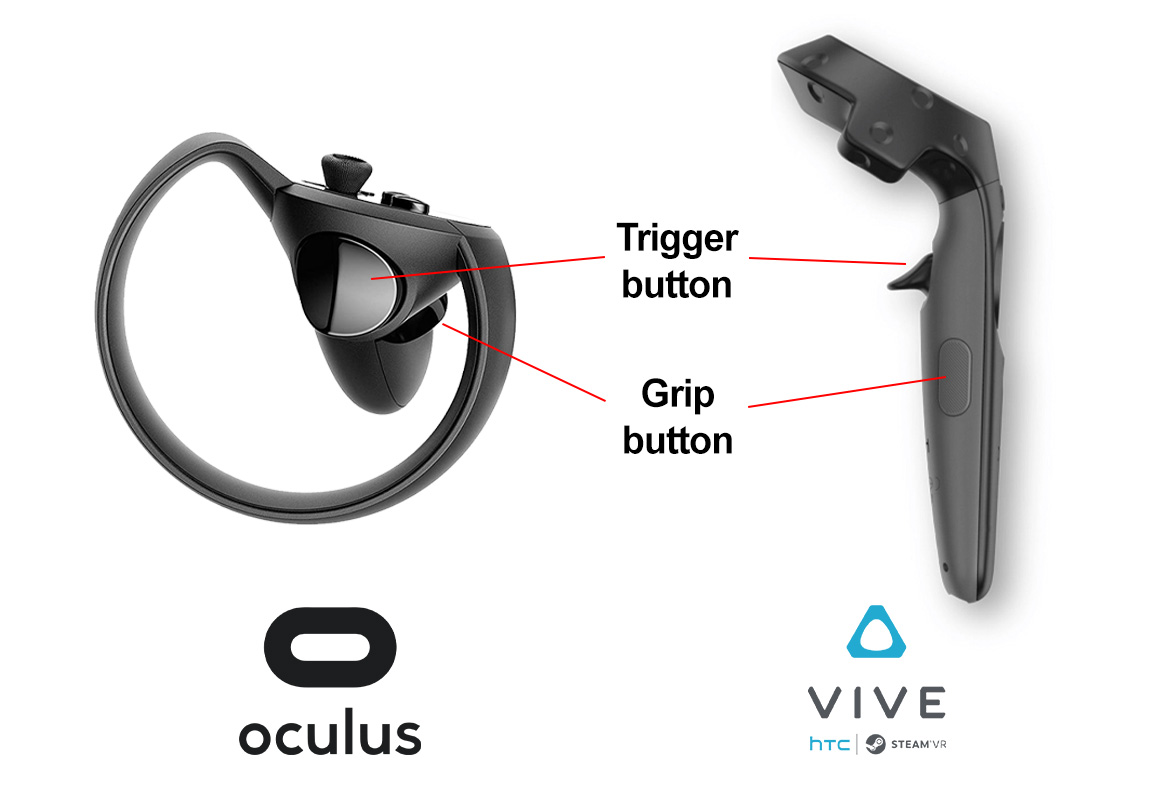
\includegraphics[width=0.9\textwidth]{figures/hand-controllers-buttons.jpg}
	\caption{Buttons on Oculus Rift and HTC Vive hand controllers, associated with common functionality in VR environment of presented software application.}
	\label{fig:hand-controllers-buttons}
\end{figure}

Trigger button can be thought of as left click on traditional computer mouse. It is used for selecting the options and moving the sliders in tablet UI component.

Grip button can be used for grabbing and moving around the simulation visualization or virtual tablet for more ergonomic interaction with the UI. To grab an object, only one of two controller's grip buttons needs to be pressed.

\subsubsection*{Running The Application}

To run a virtual reality application, no additional software has to be installed. User should run the attached executable provided on the CD, \texttt{simvr.exe}.

\subsubsection*{Virtual Reality User Interface}

After running the application, user is presented with a virtual reality environment (Figure \ref{fig:ui-annotated}).

\begin{figure}[!ht]
	\centering
	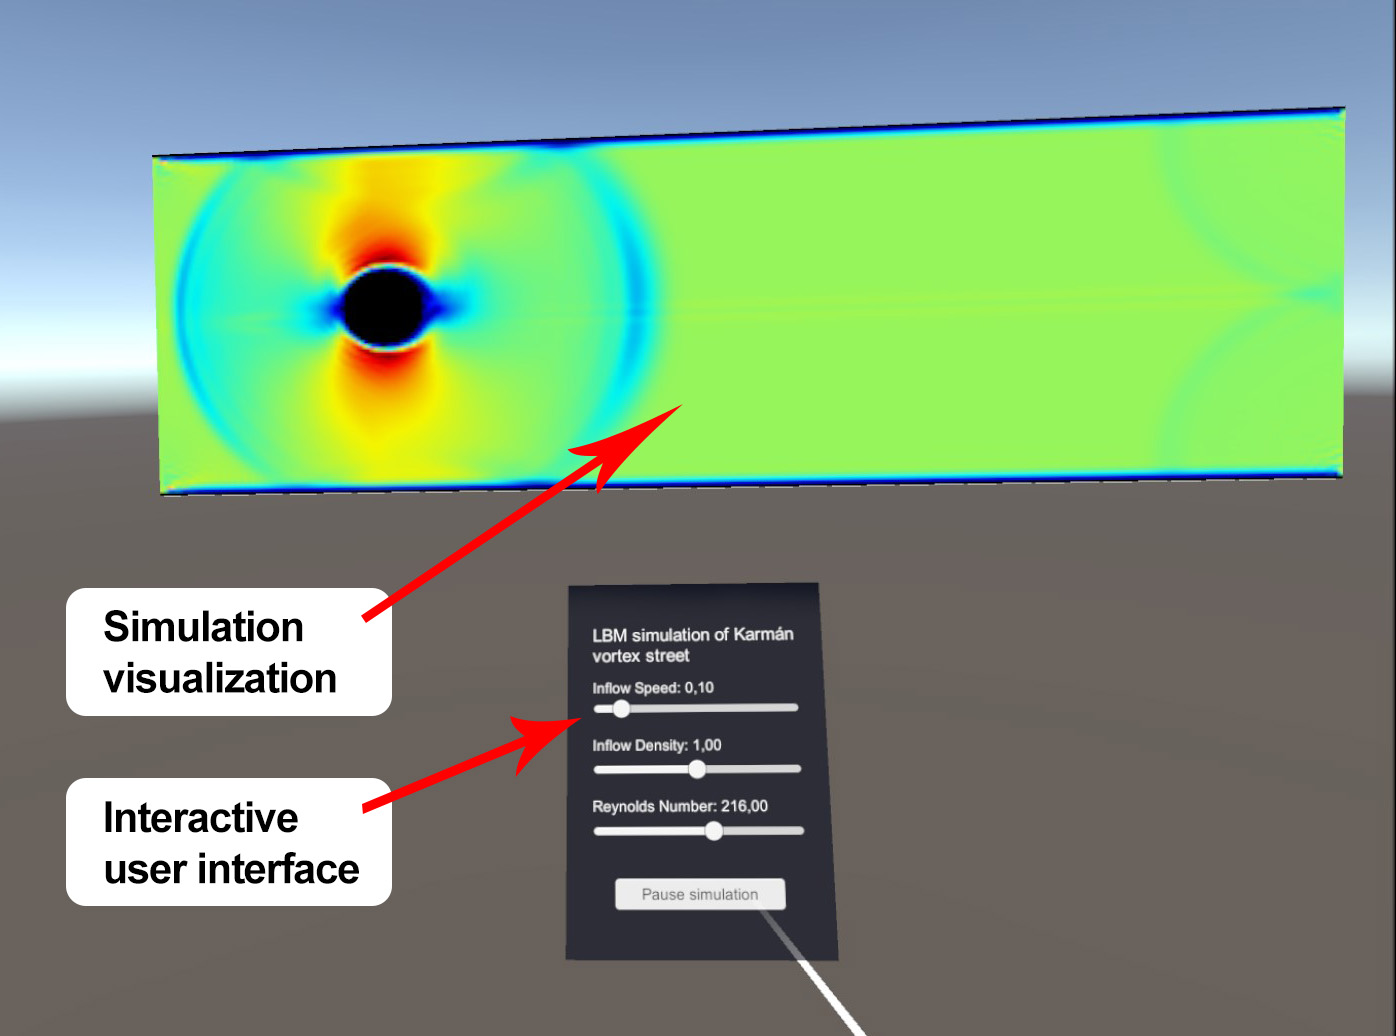
\includegraphics[width=0.9\textwidth]{figures/ui-annotated.jpg}
	\caption{Virtual reality environment.}
	\label{fig:ui-annotated}
\end{figure}

It consists of simulation visualization and a virtual ``tablet" UI to interact with the simulation. User uses VR hand controllers to point the raycaster, visualized as white ``laser", to sliders on a tablet and moves their values by sliding the circular button. To move the slider, Trigger button has to be pressed and then user can freely move it in left or right direction. It is also possible to pause and then resume simulation by pressing the button at the bottom of tablet UI.

Both simulation visualization with tablet UI can be grabbed with hand controller and moved around in any direction and rotated accordingly to user's preference. By doing this, user can reconfigure the position of both components to better suit himself. Interaction with the tablet UI can be also done by grabbing it with one hand controller (with Grip button), and interacting with it with another hand controller by pointing to it and using sliders with Trigger button\textemdash this resembles how person uses a tablet in real-life.
